\documentclass[tikz,border=4pt]{standalone}

\usepackage[T1]{fontenc}
\usepackage{newtxtext,newtxmath}
\usepackage{amsmath,amssymb}
\usetikzlibrary{arrows.meta,calc}

\begin{document}

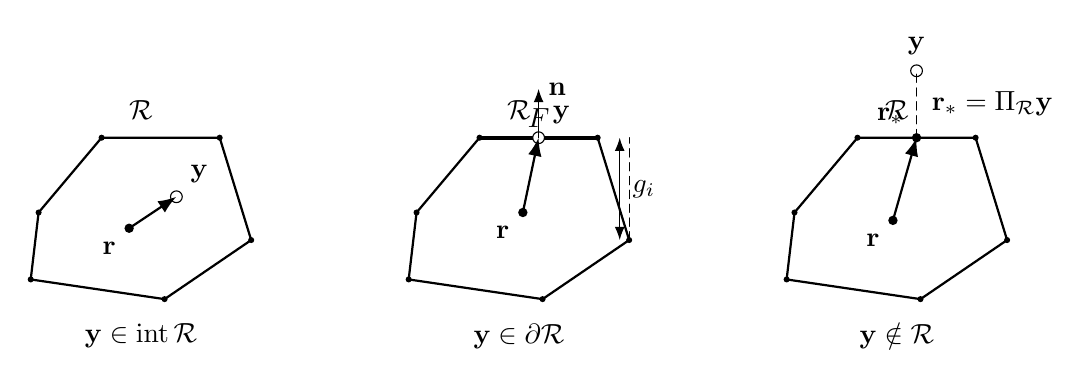
\begin{tikzpicture}[
  >=Latex,
  line cap=round,
  line join=round,
  response/.style={circle,fill,inner sep=1.2pt},
  target/.style={circle,draw,fill=white,inner sep=1.5pt},
  hull/.style={thick},
  guide/.style={densely dashed}
]

% Shared polygon:
% (0,0.4) -- (1.7,0.15) -- (2.8,0.9) -- (2.4,2.2)
% -- (0.9,2.2) -- (0.1,1.25)

% ------------------------------------------------------------------
% Interior target
% ------------------------------------------------------------------
\begin{scope}[xshift=0cm]
  \coordinate (A1) at (0,0.4);
  \coordinate (A2) at (1.7,0.15);
  \coordinate (A3) at (2.8,0.9);
  \coordinate (A4) at (2.4,2.2);
  \coordinate (A5) at (0.9,2.2);
  \coordinate (A6) at (0.1,1.25);

  \draw[hull] (A1)--(A2)--(A3)--(A4)--(A5)--(A6)--cycle;
  \foreach \P in {A1,A2,A3,A4,A5,A6}
    \fill (\P) circle (1.1pt);

  \node at (1.4,2.55) {$\mathcal R$};

  \coordinate (r) at (1.25,1.05);
  \coordinate (y) at (1.85,1.45);

  \node[response,label=below left:$\mathbf r$] at (r) {};
  \node[target,label=above right:$\mathbf y$] at (y) {};
  \draw[->,thick] (r) -- (y);

  \node[align=center] at (1.4,-0.32)
    {$\mathbf y\in\operatorname{int}\mathcal R$};
\end{scope}

% ------------------------------------------------------------------
% Boundary target
% ------------------------------------------------------------------
\begin{scope}[xshift=4.8cm]
  \coordinate (B1) at (0,0.4);
  \coordinate (B2) at (1.7,0.15);
  \coordinate (B3) at (2.8,0.9);
  \coordinate (B4) at (2.4,2.2);
  \coordinate (B5) at (0.9,2.2);
  \coordinate (B6) at (0.1,1.25);

  \draw[hull] (B1)--(B2)--(B3)--(B4)--(B5)--(B6)--cycle;
  \foreach \P in {B1,B2,B3,B4,B5,B6}
    \fill (\P) circle (1.1pt);

  \node at (1.4,2.55) {$\mathcal R$};

  \draw[line width=1.4pt] (B5)--(B4);
  \node[above] at ($(B5)!0.5!(B4)$) {$F$};

  \coordinate (r) at (1.45,1.25);
  \coordinate (y) at (1.65,2.2);
  \node[response,label=below left:$\mathbf r$] at (r) {};
  \node[target,label=above right:$\mathbf y$] at (y) {};
  \draw[->,thick] (r)--(y);

  \draw[->] (y) -- ++(0,0.62) node[right] {$\mathbf n$};

  % Normal gap of one response from the supporting hyperplane.
  \coordinate (ai) at (2.8,0.9);
  \coordinate (proj) at (2.8,2.2);
  \draw[guide] (ai)--(proj);
  \draw[<->] ($(ai)+(-0.12,0)$)--($(proj)+(-0.12,0)$);
  \node[right] at (2.72,1.55) {$g_i$};

  \node[align=center] at (1.4,-0.32)
    {$\mathbf y\in\partial\mathcal R$};
\end{scope}

% ------------------------------------------------------------------
% Exterior target
% ------------------------------------------------------------------
\begin{scope}[xshift=9.6cm]
  \coordinate (C1) at (0,0.4);
  \coordinate (C2) at (1.7,0.15);
  \coordinate (C3) at (2.8,0.9);
  \coordinate (C4) at (2.4,2.2);
  \coordinate (C5) at (0.9,2.2);
  \coordinate (C6) at (0.1,1.25);

  \draw[hull] (C1)--(C2)--(C3)--(C4)--(C5)--(C6)--cycle;
  \foreach \P in {C1,C2,C3,C4,C5,C6}
    \fill (\P) circle (1.1pt);

  \node at (1.4,2.55) {$\mathcal R$};

  \coordinate (r) at (1.35,1.15);
  \coordinate (rs) at (1.65,2.2);
  \coordinate (y) at (1.65,3.05);

  \node[response,label=below left:$\mathbf r$] at (r) {};
  \node[response,label=above left:$\mathbf r_*$] at (rs) {};
  \node[target,label=above:$\mathbf y$] at (y) {};

  \draw[->,thick] (r)--(rs);
  \draw[guide] (rs)--(y);
  \node[right] at (1.72,2.63)
    {$\mathbf r_*=\Pi_{\mathcal R}\mathbf y$};

  \node[align=center] at (1.4,-0.32)
    {$\mathbf y\notin\mathcal R$};
\end{scope}

\end{tikzpicture}

\end{document}
